\documentclass[12pt,letterpaper]{article}
\usepackage[margin=0.56in,top=0.66in,bottom=0.62in,headheight=15pt,headsep=12pt,footskip=21pt]{geometry}
\usepackage{tikz}
\usetikzlibrary{arrows.meta,calc}
\usepackage{fancyhdr,array}
\usepackage[T1]{fontenc}
\usepackage{lmodern}
\renewcommand{\familydefault}{\sfdefault}
\setlength{\parindent}{0pt}
\setlength{\parskip}{6pt}
\pagestyle{fancy}
\fancyhf{}
\renewcommand{\headrulewidth}{0.35pt}
\renewcommand{\footrulewidth}{0pt}
\newcommand{\band}[1]{\fancyhead[L]{\small Week 9 / Bouncing paths / Grades #1}}
\fancyfoot[L]{\scriptsize Bellingham Math Circle / Week 9 / F09-RV-v1}
\fancyfoot[R]{\scriptsize\thepage}
\definecolor{gridline}{gray}{0.75}
\definecolor{ray}{RGB}{32,69,115}
\tikzset{pathray/.style={draw=ray,line width=0.9pt},
         rayarrow/.style={pathray,-{Stealth[length=2.1mm]}},
         dot/.style={circle,fill=black,inner sep=1.5pt},
         finish/.style={circle,draw=black,fill=white,line width=0.8pt,inner sep=2pt}}

% All working boards use the same unit in both axes.
\newcommand{\walls}{
  \node[font=\small] at (-0.28,2) {L};
  \node[font=\small] at (4.28,2) {R};
  \node[font=\small] at (2,-0.18) {B};
  \node[font=\small] at (2,4.18) {T};}
\newcommand{\wordboard}[2]{
  \begin{tikzpicture}[x=12.5mm,y=12.5mm]
    \draw[step=1,gridline,line width=0.3pt] (0,0) grid (4,4);
    \draw[line width=0.85pt] (0,0) rectangle (4,4);
    \walls
    \node[dot] at (1,1) {};
    \node[font=\small,anchor=north east] at (0.94,0.95) {S};
    \node[finish] at (#1,3) {};
    \node[font=\small,anchor=south west] at (#1+0.10,3.03) {F};
    \node[font=\small,anchor=south] at (2,4.55) {Finish #2};
    \node[font=\small,anchor=north] at (2,-0.46) {Word: \rule{17mm}{0.35pt}};
  \end{tikzpicture}}
\newcommand{\pairboards}{
  \begin{minipage}[t]{0.49\textwidth}\centering\wordboard{2}{A}\end{minipage}\hfill
  \begin{minipage}[t]{0.49\textwidth}\centering\wordboard{3}{B}\end{minipage}}

\newcommand{\counterboard}[2]{
  \begin{tikzpicture}[x=#1mm,y=#1mm]
    \draw[step=1,gridline,line width=0.35pt] (0,0) grid (6,4);
    \draw[line width=0.9pt] (0,0) rectangle (6,4);
    \ifnum#2=1
      \foreach \x/\y/\letter in {1/3/A,2/3/B,3/3/C,4/3/D,5/3/E,1/2/F,2/2/G,3/2/H,4/2/I,5/2/J,1/1/K,2/1/L,3/1/M,4/1/N,5/1/O}{
        \node[dot] at (\x,\y) {};
        \node[font=\small,anchor=north west,fill=white,inner sep=0.6pt] at (\x+0.05,\y-0.05) {\letter};}
    \fi
  \end{tikzpicture}}

\newcommand{\crossboard}[2]{
  \begin{tikzpicture}[x=12.5mm,y=12.5mm]
    \draw[step=1,gridline,line width=0.35pt] (0,0) grid (#1,#2);
    \draw[line width=0.9pt] (0,0) rectangle (#1,#2);
    \node[dot] at (0,0) {};
    \draw[rayarrow] (0,0)--(0.48,0.48);
    \node[font=\small,anchor=north east] at (-0.07,-0.07) {S};
    \node[font=\small,anchor=south] at (#1/2,#2+0.22) {#1 wide, #2 high};
    \node[font=\small,anchor=north] at (#1/2,-0.65) {Crossings: \rule{12mm}{0.35pt}};
  \end{tikzpicture}}

\begin{document}
\band{2--5}
Each path travels straight between walls. At a bounce, the two angles to the wall
are equal. A path stops if it hits a corner. The walls are left L, right R,
bottom B and top T.

\begin{center}
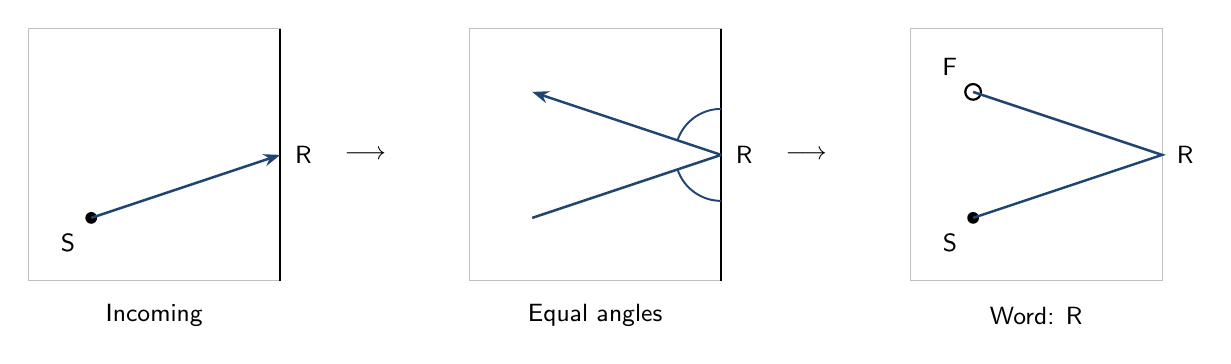
\begin{tikzpicture}[x=8mm,y=8mm,font=\small]
  % A non-task one-bounce example: S=(1,1), R=(4,2), F=(1,3).
  \begin{scope}
    \draw[gridline] (0,0) rectangle (4,4);
    \draw[line width=0.9pt] (4,0)--(4,4);
    \node[dot] at (1,1) {};
    \node[anchor=north east] at (0.9,0.9) {S};
    \draw[rayarrow] (1,1)--(4,2);
    \node[anchor=west] at (4.08,2) {R};
    \node at (2,-0.55) {Incoming};
  \end{scope}
  \node at (5.35,2) {$\longrightarrow$};
  \begin{scope}[shift={(7,0)}]
    \draw[gridline] (0,0) rectangle (4,4);
    \draw[line width=0.9pt] (4,0)--(4,4);
    \draw[pathray] (1,1)--(4,2);
    \draw[rayarrow] (4,2)--(1,3);
    \draw[ray,line width=0.7pt] (4,1.27) arc[start angle=-90,end angle=-161.565,radius=0.73];
    \draw[ray,line width=0.7pt] (3.307,2.231) arc[start angle=161.565,end angle=90,radius=0.73];
    \node[anchor=west] at (4.08,2) {R};
    \node at (2,-0.55) {Equal angles};
  \end{scope}
  \node at (12.35,2) {$\longrightarrow$};
  \begin{scope}[shift={(14,0)}]
    \draw[gridline] (0,0) rectangle (4,4);
    \node[dot] at (1,1) {};
    \node[finish] at (1,3) {};
    \node[anchor=north east] at (0.9,0.9) {S};
    \node[anchor=south east] at (0.9,3.1) {F};
    \draw[pathray] (1,1)--(4,2)--(1,3);
    \node[anchor=west] at (4.08,2) {R};
    \node at (2,-0.55) {Word: R};
  \end{scope}
\end{tikzpicture}
\end{center}

Write wall names in the order touched: LR means left, then right.

\textbf{Problem 1:} Find every wall word that gets from S to F with exactly
two bounces. Find the words for both finishes. A word may use the same wall twice,
if a path can do it. Draw each path with a ruler.

\vspace{3pt}
\pairboards
\vspace{5pt}
\pairboards

\newpage
\band{2--5}
Extra workspace for Problem 1.

Finish A words: \hrulefill

Finish B words: \hrulefill

\pairboards
\vspace{4pt}
\pairboards
\vspace{4pt}
\pairboards

\newpage
\band{2--5}
Extra workspace for Problem 1.

\pairboards
\vspace{4pt}
\pairboards
\vspace{4pt}
\pairboards

\newpage
\band{4--5}
For diagonal paths, move one square across and one square up or down each step.
Keep the counter's arrow pointing along its next move. At a wall, turn the arrow
away from that wall. Stop at a corner.

\begin{center}
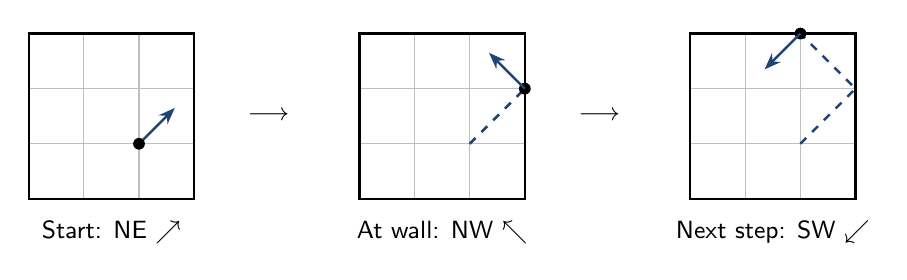
\begin{tikzpicture}[x=7mm,y=7mm,font=\small]
  \begin{scope}
    \draw[step=1,gridline] (0,0) grid (3,3);
    \draw[line width=0.8pt] (0,0) rectangle (3,3);
    \draw[rayarrow] (2,1)--(2.65,1.65);
    \node[dot] at (2,1) {};
    \node at (1.5,-0.6) {Start: NE $\nearrow$};
  \end{scope}
  \node at (4.35,1.5) {$\longrightarrow$};
  \begin{scope}[shift={(6,0)}]
    \draw[step=1,gridline] (0,0) grid (3,3);
    \draw[line width=0.8pt] (0,0) rectangle (3,3);
    \draw[pathray,dashed] (2,1)--(3,2);
    \node[dot] at (3,2) {};
    \draw[rayarrow] (3,2)--(2.35,2.65);
    \node at (1.5,-0.6) {At wall: NW $\nwarrow$};
  \end{scope}
  \node at (10.35,1.5) {$\longrightarrow$};
  \begin{scope}[shift={(12,0)}]
    \draw[step=1,gridline] (0,0) grid (3,3);
    \draw[line width=0.8pt] (0,0) rectangle (3,3);
    \draw[pathray,dashed] (2,1)--(3,2)--(2,3);
    \node[dot] at (2,3) {};
    \draw[rayarrow] (2,3)--(1.35,2.35);
    \node at (1.5,-0.6) {Next step: SW $\swarrow$};
  \end{scope}
\end{tikzpicture}
\end{center}

\textbf{Problem 2:} Start at each lettered dot, with the arrow pointing NE $\nearrow$.
Which starts reach a corner? Which return to their starting dot with the arrow
pointing NE $\nearrow$? Mark C for a corner and L for a loop. For each loop, find
the number of diagonal steps until that first return.

\begin{center}\counterboard{22}{1}\end{center}

\begin{center}
\renewcommand{\arraystretch}{1.7}
\begin{tabular}{*{5}{>{\centering\arraybackslash}p{28mm}}}
A \rule{12mm}{0.35pt} & B \rule{12mm}{0.35pt} & C \rule{12mm}{0.35pt} & D \rule{12mm}{0.35pt} & E \rule{12mm}{0.35pt}\\
F \rule{12mm}{0.35pt} & G \rule{12mm}{0.35pt} & H \rule{12mm}{0.35pt} & I \rule{12mm}{0.35pt} & J \rule{12mm}{0.35pt}\\
K \rule{12mm}{0.35pt} & L \rule{12mm}{0.35pt} & M \rule{12mm}{0.35pt} & N \rule{12mm}{0.35pt} & O \rule{12mm}{0.35pt}
\end{tabular}
\end{center}

Loop starts and their step counts: \hrulefill

\vspace{9pt}\hrulefill

\newpage
\band{4--5}
Extra workspace for Problem 2.

\begin{center}
\counterboard{18}{0}\\[2pt]
Starting letter: \rule{12mm}{0.35pt}\qquad Loop steps: \rule{15mm}{0.35pt}

\vspace{5pt}
\counterboard{18}{0}\\[2pt]
Starting letter: \rule{12mm}{0.35pt}\qquad Loop steps: \rule{15mm}{0.35pt}

\end{center}

\newpage
\band{2--5}
For diagonal paths, move one square across and one square up or down each step.
A crossing is one place inside the board where two pieces of the path form an X.
Wall hits and corners do not count.

\begin{center}
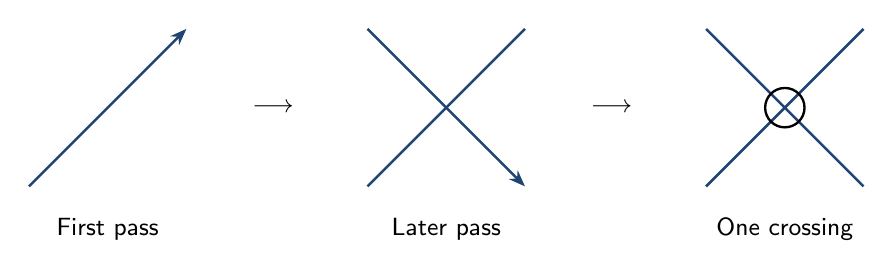
\begin{tikzpicture}[x=10mm,y=10mm,font=\small]
  \begin{scope}
    \draw[rayarrow] (0,0)--(2,2);
    \node at (1,-0.55) {First pass};
  \end{scope}
  \node at (3.1,1) {$\longrightarrow$};
  \begin{scope}[shift={(4.3,0)}]
    \draw[pathray] (0,0)--(2,2);
    \draw[rayarrow] (0,2)--(2,0);
    \node at (1,-0.55) {Later pass};
  \end{scope}
  \node at (7.4,1) {$\longrightarrow$};
  \begin{scope}[shift={(8.6,0)}]
    \draw[pathray] (0,0)--(2,2) (0,2)--(2,0);
    \draw[line width=0.85pt] (1,1) circle (0.25);
    \node at (1,-0.55) {One crossing};
  \end{scope}
\end{tikzpicture}
\end{center}

\textbf{Problem 3:} Start at S heading NE $\nearrow$ and draw each diagonal path
until it reaches a corner. Circle its crossing points. Which boards have the same
number of crossings? Find a rectangle with exactly ten crossings on the next page.

\begin{center}
\begin{minipage}[b]{0.49\textwidth}\centering\crossboard{2}{3}\end{minipage}\hfill
\begin{minipage}[b]{0.49\textwidth}\centering\crossboard{3}{4}\end{minipage}

\vspace{10pt}
\begin{minipage}[b]{0.49\textwidth}\centering\crossboard{4}{5}\end{minipage}\hfill
\begin{minipage}[b]{0.49\textwidth}\centering\crossboard{4}{6}\end{minipage}
\end{center}

\newpage
\band{2--5}
Extra workspace for Problem 3. Outline your rectangle on the grid.

\begin{center}
\begin{tikzpicture}[x=12.5mm,y=12.5mm]
  \draw[step=1,gridline,line width=0.35pt] (0,0) grid (12,12);
  \node[dot] at (0,0) {};
  \node[font=\small,anchor=north east] at (-0.07,-0.07) {S};
  \draw[rayarrow] (0,0)--(0.48,0.48);
\end{tikzpicture}
\end{center}

My rectangle: \rule{20mm}{0.35pt} wide, \rule{20mm}{0.35pt} high.

Crossings: \rule{20mm}{0.35pt}

\vfill
\end{document}
